\documentclass[a4paper, 12pt]{article}

\usepackage[utf8]{inputenc}
\usepackage[T1]{fontenc}
\usepackage[english, francais]{babel}
\usepackage{graphicx}
\usepackage{listings}
\usepackage{color}
 
\definecolor{codegreen}{rgb}{0,0.6,0}
\definecolor{codegray}{rgb}{0.5,0.5,0.5}
\definecolor{codepurple}{rgb}{0.58,0,0.82}
\definecolor{backcolour}{rgb}{0.95,0.95,0.92}

\lstdefinestyle{mystyle}{
    backgroundcolor=\color{backcolour},   
    commentstyle=\color{codegreen},
    keywordstyle=\color{magenta},
    numberstyle=\tiny\color{codegray},
    stringstyle=\color{codepurple},
    basicstyle=\footnotesize,
    breakatwhitespace=false,         
    breaklines=true,                 
    captionpos=b,                    
    keepspaces=true,                 
    numbers=left,                    
    numbersep=5pt,                  
    showspaces=false,                
    showstringspaces=false,
    showtabs=false,                  
    tabsize=2
}

\lstset{language=C++,
    basicstyle=\small,
    keywordstyle=\color{blue}\small,
    stringstyle=\color{red}\small,
    commentstyle=\color{green}\small,
    morecomment=[l][\color{magenta}]{\#},
    tabsize=2
}
\title{Le vouitris}
\date{?? mars 2019}
\author{Cynthia MAILLARD \and Alexandre DILLON \and Félix ROYER}

\begin{document}

\maketitle

\newpage

\tableofcontents

\newpage

\section*{Remerciements}
	
\section*{Introduction}
	La réalisation de ce projet s'inscrit dans le cadre du projet intégrateur de notre troisième année de licence informatique à l'Université de Besançon. Pour ce projet, nous avons réalisé le sujet proposé par Julien Bernard, enseignant-chercheur en informatique à l'Université de Franche-Comté : un tétris multijoueur en réseau. 

	\bigskip

	Le développement devait être fait en C++, avec le bibliothèque Boost.asio pour la communication réseau et les parties graphiques devait être réalisées en utilisant la biliothèque Gamedev Framework, biliothèque conçu pour le développement de jeux vidéo, développée par Julien Bernard.
	Le développement s'étendait d'octobre 2018 à mars 2019.

	\bigskip
	Nous étions intéressé par ce projet car nous voulions améliorer nos connaissances dans le language C++. De plus la simplicité de la conception d'un Tétris nous permettait d'approfondir certains domaines que le court temps de développement ne nous aurait pas permi d'aborder sur un jeu plus complexe. Notamment, approfondir la programmation distribué et la sérialization nous motivait pour ce projet.

	\bigskip
	Ce rapport a pour but de rendre compte du travail que nous avons réalisé au cours du projet.

	\newpage

\section{Adaptation du jeu d'origine}
	\subsection{Tétris originel}
		Tetris est un jeu vidéo de puzzle conçu par Alekseï Pajitnov en 1984. Tetris est principalement composé d'une zone de jeu où des pièces de formes différentes, appelées « tétriminos », descendent du haut de l'écran. 
		Durant la chute des tetrominos, le joueur peut déplacer les pièces latéralement, leur faire effectuer une rotation sur elles-mêmes et accélérer la vitesse de la descente dans certaines versions jusqu'à ce qu'elles se pose sur le bas de la zone de jeu ou sur une autre pièce. 
		Le but pour le joueur est de réaliser le plus de lignes possibles. Une fois une ligne complétée, elle disparaît, et les blocs placés au-dessus chutent d'un rang. 
		Lorsque le joueur accumule les pièce et remplie la zone de jeu jusqu’en haut, ce qui empêche l'arrivée de tétriminos supplémentaires, la partie se termine. Le joueur obtient un score, qui dépend essentiellement du nombre de lignes réalisées lors de la partie. On ne peut donc jamais gagner à Tetris, le but étant d’améliorer son précédent score.

		Après la version originale du jeu sortie sur l'\textit{Elektronika 60}, le tétris a connu un succès mondial dans les années 1990 grâce à sa version Gameboy.

		Le jeu a été adapté sur pratiquement toutes les consoles de toutes les générations, soit dans une version strictement identique soit dans une adaptation plus libre ne conservant que certains point du gameplay original. Au début des années 2010, on comptait plus de 65 plate-formes qui possaidait un portage du jeu.

		Tétris s'est imposé comme l'un des plus grands succès de l'histoire du jeu vidéo et l'une de ces icones les plus mondialement connues. Il faut noter également que le jeu a connue des adaptations multijoueurs - notamment le projet \emph{Tétrinet} à la fin des années 1990 - et ce encore aujourd'hui, avec par exemple \emph{Tétris 99}, qui est sorti le 13 février 2019 sur Nintendo Switch.

	\subsection{Notre adaptation}
		Notre adaptation est une version multijoueur du Tétris, où chaque joueur a un jeu qui tourne sur son ordinateur, sur lequel il joue seul avec son clavier. 

		L'objectif hypotétique étant que pour jouer ensemble, deux joueurs puissent télécharger le client du jeu sur leurs ordinateur puis se connectent à un serveur en ligne qui gérerait le déroulement de la partie. 
		Ainsi, on pourrait imaginer que le joueur rédeveloppe son propre client avec son propre interface graphique, et il pourrait jouer sans problème, à condition de reproduire les échanges entre le client et le serveur prévus dans le protocole.

		Cette proposition pésente le risque qu'un joueur recode sa version du client et soit donc capable de tricher, car n'étant plus contraint aux même règles que son adversaire.

		Cela nous a donné une contrainte à respecter : le serveur fait loi. Les clients ne servent qu'à l'affichage du jeu et à la réception des actions de l'utilisateur, mais ne contrôlent pas le déroulement de la partie.

		Les joueurs joueront une partie de Tétris classique, chacun de leur coté. Cependant, pour ne pas limiter l'affrontement à un concours de score, nous avons choisi d'ajouter un système de malus : lorsqu'un joueur parvient à détruire des lignes, son adversaires se voit pénalisé plus ou moins sévérement en fonction du nombre de lignes détruites.

	\section{Modélisation du jeu}

		\subsection{Architecture réseau}

			Nous avons déjà défini que nous avions besoin d'une architecture client-serveur dans la partie précédente.

			Un problème que nous avons rencontré est que les clients et le serveur doivent être capable d'attendre l'arrivé d'un message sur leur socket, tout en exécutant une boucle simultanément - la fenêtre graphique pour les clients et la boucle de jeu pour le serveur.


			Pour résoudre ce problèmes nous avons séparé la réception des messages dans un thread à part dans les clients et le serveur.

			Ce thread attends la reception d'un message et le place dans une file. Le thread principal récupère ensuite les messages contenu dans cette file et les exploitent, comme on peut le voir sur la figure \ref{fig:rezo}.

			\begin{figure}[bt]
				\centering
				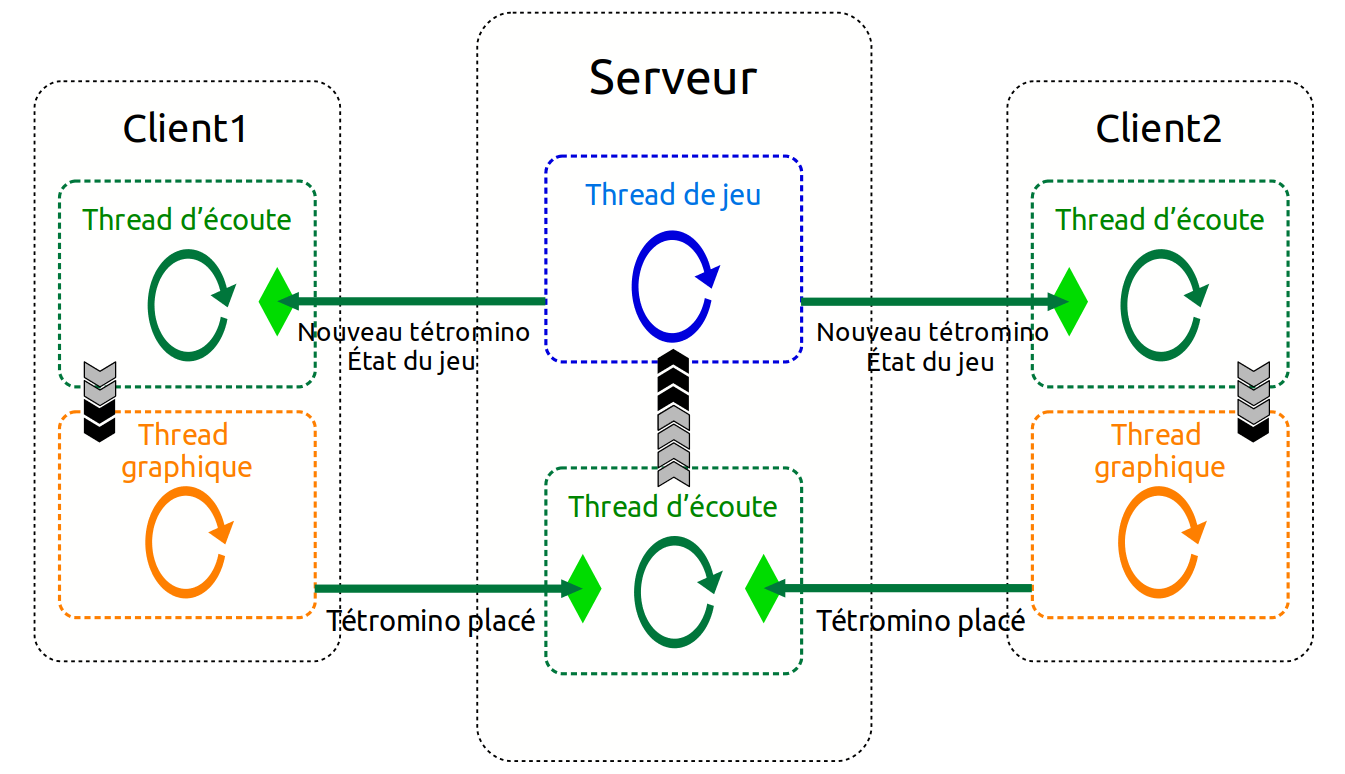
\includegraphics[scale=0.35]{img/archi_reseau.png}
				\caption{Représentation simplifiée de l'architecture réseau entre les clients et le serveur}
				\label{fig:rezo}
			\end{figure}

			Ainsi, les clients et le serveur vont pouvoir s'envoyer des messages sans problèmes, étant donné qu'il y a en permanence une socket qui écoute la réception de message. L'interprétation des messages est faites durant la boucle principale des deux applications, ce qui ne bloque pas leur exécution.

		\subsection{\'Echanges entre les clients et le serveur}

			Notre protocole d'échange tel que l'avons défini implique que le serveur gère seul la partie, et les clients uniquement l'affichage et les interactions de l'utilisateur, par conséquent, les échanges vont consister en la mise à jour de l'état du jeu de la part du serveur et les actions du joueur de la part du client. 
			La figure \ref{fig:echange} représente une version simplifié des échanges entre les clients et le serveur. Pour des soucis de lisibilité, nous avons assumé que seul le premier joueur place des tétrominos.

			\begin{figure}[bt]
				\centering
				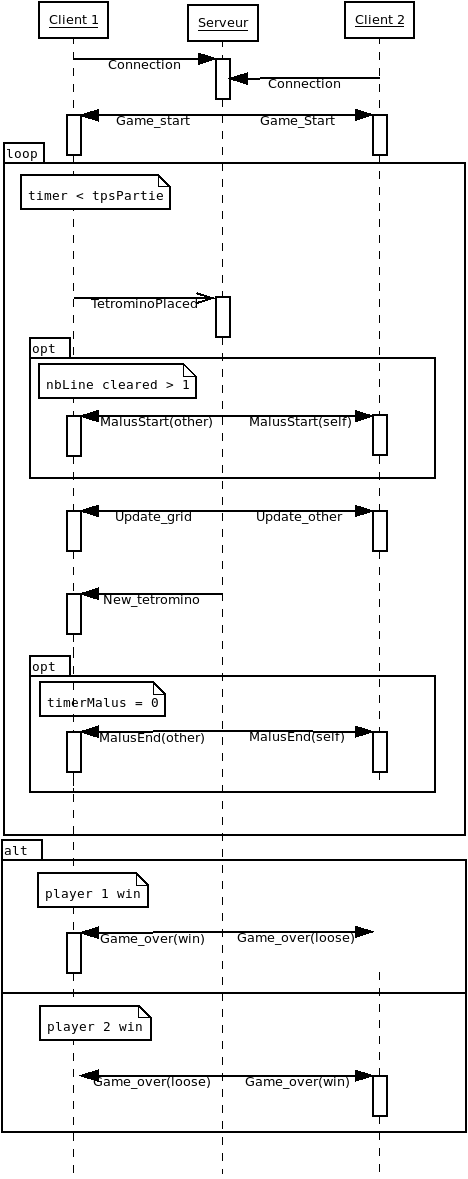
\includegraphics[scale=0.45]{img/echanges.png}
				\caption{Représentation simplifiée des échanges de messages entre les clients et le serveur}
				\label{fig:echange}
			\end{figure}


			\subsubsection{Les messages du serveur vers le client}

				\begin{itemize}
					\item Game start : message de début de partie, signale le début de la partie aux clients lorsque les deux joueurs sont prêts à jouer
					\item Game over : message de fin de partie, il indique au joueur s'il a gagné, perdu ou s'il y a une égalité
					\item New tetromino : message contenant le prochaine tétromino qui sera utilisé par le client
					\item Update Grid : message qui contient la grille de jeu du joueur
					\item Update Other Grid : message qui contient la grille de l'adversaire, pour l'afficher
					\item Malus start : signale le début d'une période malus pour le joueur ainsi que le type du malus qui s'applique
					\item Malus end : signale la fin de la période de malus actuelle
				\end{itemize}

			\subsubsection{Les messages du client vers le serveur}

				\begin{itemize}
					\item Tétromino placed : contient le tétromino avec sa position et son orientation tel qu'il viens d'être placé par le joueur
					\item Connection lost : message signalant une déconnexion du joueur
				\end{itemize}




\section{Mise en oeuvre}
	\subsection{Le serveur}

		Le serveur est la clé de voute du jeu. Il fait le lien entre les deux clients et gère l'évolutions du jeu.

		\subsubsection{La structure du serveur}

			\paragraph{Les threads}

			Le serveur doit écouter les messages de la part des deux clients. Cependant, l'éxecution du serveur ne peut être interomput en attendant la reception d'un message. Nous avons donc créé deux threads d'écoute, chacun attendant les message d'un des client. Lors qu'un message est réceptionné, il est stocké dans une file. La file est partagée entre le thread d'écoute et le thread principal. \'A chaque tour de boucle, le thread principal regarde s'il y a un message stocké dans le file. Si c'est le cas, il interprète ce dernier, met à jour les données du client et renvoit des message aux deux clients si besoin est.


			\paragraph{L'interprétation des messages}

				


		\subsubsection{Les malus}


			Présentation des différents malus:

			Lorsque le joueur complète des lignes, celle ci sont supprimés. On calcul le nombre de lignes supprimé afin d’augmenté le score du joueur mais aussi d’envoyé des malus au joueur adverse.
			Pour les malus nous avons choisis : 

			\begin{itemize}
				\item suppression de 2 lignes : le joueur adverse ne peut plus faire de rotation sur ses pièces pendant N secondes.
				\item suppression de 3 lignes : la vitesse des chutes des pièce de l’adversaire augmente.
				\item suppression de 4 lignes : certaines case sont enlevé du mur adverse pouvant l’empêcher de compléter certaine lignes.
			\end{itemize}

			Transmission des messages pour les malus ?






	\subsection{La sérialisation}

		Les échanges des messages vus précédemment nécessite une sérialisation afin qu'ils puissent être envoyés par les sockets, ces dernières ne pouvant envoyés que des tableaux d'octet.


		Pour ce projet, nous avons réalisé nos propres classes de sérialisation. Nous nous sommes inspirés des bibliothèques de sérialisation de GamedevFramework ainsi que de SFML/Packet. 
		Notre sérialisation est organisée en deux classe symétrique : Serializer et Deserializer. Elles contiennent tous les deux un tableau dynamique d'octet qui représente les informations sérialisés ainsi qu'une position d'écriture ou de lecture, respectivement pour le serialiseur et le deserialiseur. 
		
		\subsubsection{Sérialisation des types simples}

		Pour la sérailisation des type simple nous utilisons une méthode templatée privée qui peut sérialiser n'importe quel type simple. Cet sérialisation est ensuite appelé par d'autre méthode auxquelles sont assignés des types spécifiques afin d'éviter la sérialisation de type non-désiré.

		
		L'endianess de cet méthode de sérialisation, c'est-à-dire l'ordre sequentiel dans lequel sont ranger nos données sérialisées, définit l'endianess de toute notre sérialisation, celle-ci est au format big-endian pusique celui-ci est le format le plus commun au infrastructure réseau. Cela signifie que l'octet le plus significatif (octet de poid fort) est stocker en premier dans notre sérialisation et est donc envoyé en premier lors des échanges.

\begin{lstlisting}[language=C++, caption=Méthode de sérailisation de type simple\, data est notre tableau dynamique\, d la varaible de type T à sérailiser et writePos la position d'écriture du sérialiseur]
template <typename T>
void Serializer::serializeAnyType(T d){
	size_t size = sizeof(T);
	for (size_t i = 0; i < size; ++i) {
		data.push_back(static_cast<uint8_t>(d >> 8*(size-i-1))); 
	}
	writePos += sizeof(T);
}\end{lstlisting}

\begin{figure}[bt]
	\centering
	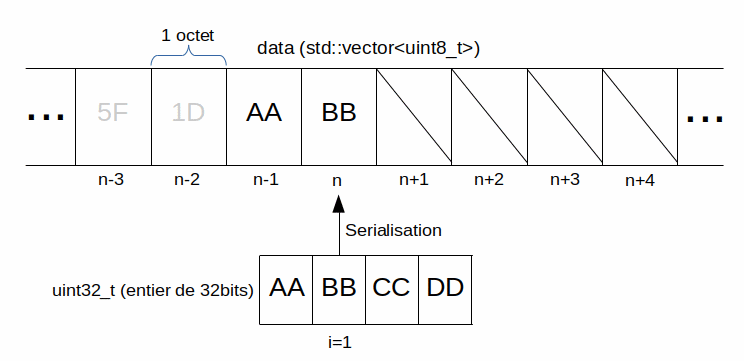
\includegraphics[scale=0.35]{img/serialisation.png}
	\caption{Représentation simplifiée de la sérialisation d'un entier de 32bit, est ici représenté la sérialisation du second octet avec la position d'écriture égale à n.}
	\label{fig:serial}
\end{figure}

			\subsubsection{La sérialisation des messages}

			Nos messages sont répartis en deux structures, une pour les échanges client vers serveur et une pour les échanges serveur vers client. Chacune de ces structures contient une union contenant les structures des messages ainsi que le type du message représenté par une énumération.


			Les structures de messages contiennent ensuite ce que chaque message doit envoyer, des types simples ou des objets. La sérialisation des types simples étant réalisée, celles des objets ce fait par l'appel de la sérailisation de types simple pour chaque attribut de l'objet, sauf si l'attribut est lui-même un objet pour lequel on appelera la méthode de sérialisation adéquate, ceci jusqu'à la sérialisation complète de tout l'objet.
			

			La sérialisation des messages est donc la suivante : on sérialise tout d'aboord le type de message puis la structure de message présente dans l'union correspondante au type du message.

			\subsubsection{La déserialisation}

			Comme précédemment évoquer, le Deserializer est le symétrique du Serializer, de ce fait la déserialisation va effectuer les opérations inverse de la sérialisation. Pour le cas des messages, le Deserializer va d'abord déserialiser la type du message pour savoir quelle methode appeler pour deserialiser le message.

\begin{lstlisting}[language=C++, caption=Méthode de desérailisation de type simple\, data est notre tableau dynamique\, d la varaible de type T à desérailiser et readPos la position de lecture du desérialiseur]
template <typename T>
void Deserializer::deserializeAnyType(T & d){
	T res = 0;
	for (size_t i = 0; i < sizeof(T); ++i) {
		res = (res << 8) + data[readPos+i];
	}
	readPos += sizeof(T);
	d = res;
}\end{lstlisting}

			\subsubsection{Une seule asymétrie entre Serializer et Deserializer}

			Une seule asymétrie entre Serializer et Deserializer existe, il s'agit de la gestion de la taille du message. Car pour envoyé notre message sur une socket, nous devons connaitre sa taille et la spécifier. Pour cela le serialiseur garde toujours huit octets en debut de son tableau dynamique pour que lorsqu'on récupère le tableau d'octet, la taille du tableau soit insérée au debut de celui-ci. Ainsi cela permet lors de la réception du message, de lire les huit premiers octets pour connaitre la taille du message et alloué un tableau dynamique de la bonne taille pour enfin l'assigné à un deserailiseur.

	
	\subsection{Les structures de données communes}

		\subsubsection{Tetromino}

			crée a quel moment ?

			L’objet de la classe Tétromino contient les informations sur le tetromino actuellement en jeu :
			\begin{itemize}
				\item son type
				\item son sens de rotation actuel
				\item sa forme représenté pas une matrice de 4x2
				\item la position de son ancre représenté par un vecteur (x, y)
			\end{itemize}

			Explication des getter et setter ??

			La fonction Tetromino::getCases permet de récupérer la [liste] a modifier, des vecteur représentant les coordonnées de toute les cases du tetromino en fonction de sa rotation, de sa forme et de la position de l’ancre.

		\subsubsection{Grid}
			Pour représenter la zone de jeu nous utilisons un tableau d’entier à une dimension. Une case vide est représenté par un 0. 
			On crée le tableau avec l’objet Grid.

			Fonction dans Grid :

			les constructeur besoin d’en parler ?
			IsValid ??
			printGrid -> debug , besoin d’en parler ?

			\paragraph{Vérification des déplacements}
				La fonction Grid::movePossible permet de vérifier si l’action de déplacement faite par le joueur et valide. Elle prend en paramètre le Tétromino en jeu (tetromino qui chute et qui est contrôlé par le joueur) et un vecteur (x, y) pour savoir dans quel direction le mouvement est fait.

				Cette fonction est appelé dans : 
				\begin{itemize}
					\item Grid::downPossible, avec le vecteur {0, 1}
					\item Grid::rightPossible, avec le vecteur {1, 0}
					\item Grid::leftPossible, avec le vecteur {-1, 0}
				\end{itemize}

				La fonction Grid::rotatePossible permet d’autorisé où non la rotation de la pièce en jeu. La rotation peut être par exemple refusé si le tetromino est bloqué entre 2 autres tétrominos ou si il est sur le bord de la zone de jeu. Dans ces 2 cas, la rotation du tétromino le ferait soit passé a travers d’autre pièce ce qui est impossible ou encore sortir de la zone de jeu. On vérifie donc si les case du tétromino après rotation sont bien dans la zone de jeu et si elle sont vide grâce à la fonction Tetromino::getCases.

			\paragraph{Placement d’un tetromino}
				Si la fonction Grid::downPossible renvoie false, le tetromino actuellement en jeu est placé. Hors, seul son ancre est visible dans le tableau lors de sa chute, il faut donc ajouter toute les cases qui compose le tetromino dans la zone de jeu afin d’envoyé un nouveau tetromino en jeu.
				On appel la fonction Grid::printGrid qui remplis le tableau en faisant appel au fonction Tetromino::getCases et Tetromino::getType.

			\paragraph{Suppression de lignes}
				La fonction Grid::deleteLines parcours le tableau et détecte si des lignes sont pleine.
				Si c’est le cas, elle appel la fonction Grid::fallLines sur la lignes correspondante.
				Elle renvoie le nombre total de ligne pleine qui ont été supprimé pour effectué le calcul du score et l’envoie de malus à l’adversaire.

				La fonction Grid::fallLines récupère en paramètre la ligne pleine, et fait descendre toutes les lignes au dessus de celle-ci d’une case vers le bas en commençant par le bas du tableau.

			\paragraph{Vérification de l’état de la grille}

				La fonction Grid::gameOver est appelé à chaque tétromino posé. Elle vérifie si les lignes du haut du tableau sont vide. Si une pièce est présente dans cette zone, on estime que la zone de jeu est complètement remplis et que l’arrive d’un prochain tétromino est impossible, dans ce cas elle renvoie true.

			\paragraph{clear (titre a changer)}

				Si l’appel à la fonction Grid::gameOver nous retourne true alors on vide entièrement la zone de jeu et le score du joueur subit un malus (score divisé par 2). 
				Pour vidé la zone de jeu on utilise la fonction Grid::clear qui parcours tout le tableau est passe tout les case à 0.



	\subsection{Le client graphique}

		Le client est la partie visible de l’application pour les joueurs. Son rôle est de recevoir les messages envoyé par le serveur, de capter les interaction du joueur sur la partie et de les transmettre au server et d’afficher les différents éléments composant la fenêtre de jeu.

		\subsubsection{Les structures de données locales}

			%les données stockés dans le clients, 
			%comment elles ont mises à joru par les messages du serveur
			%

			\begin{figure}[bt]
				\centering
				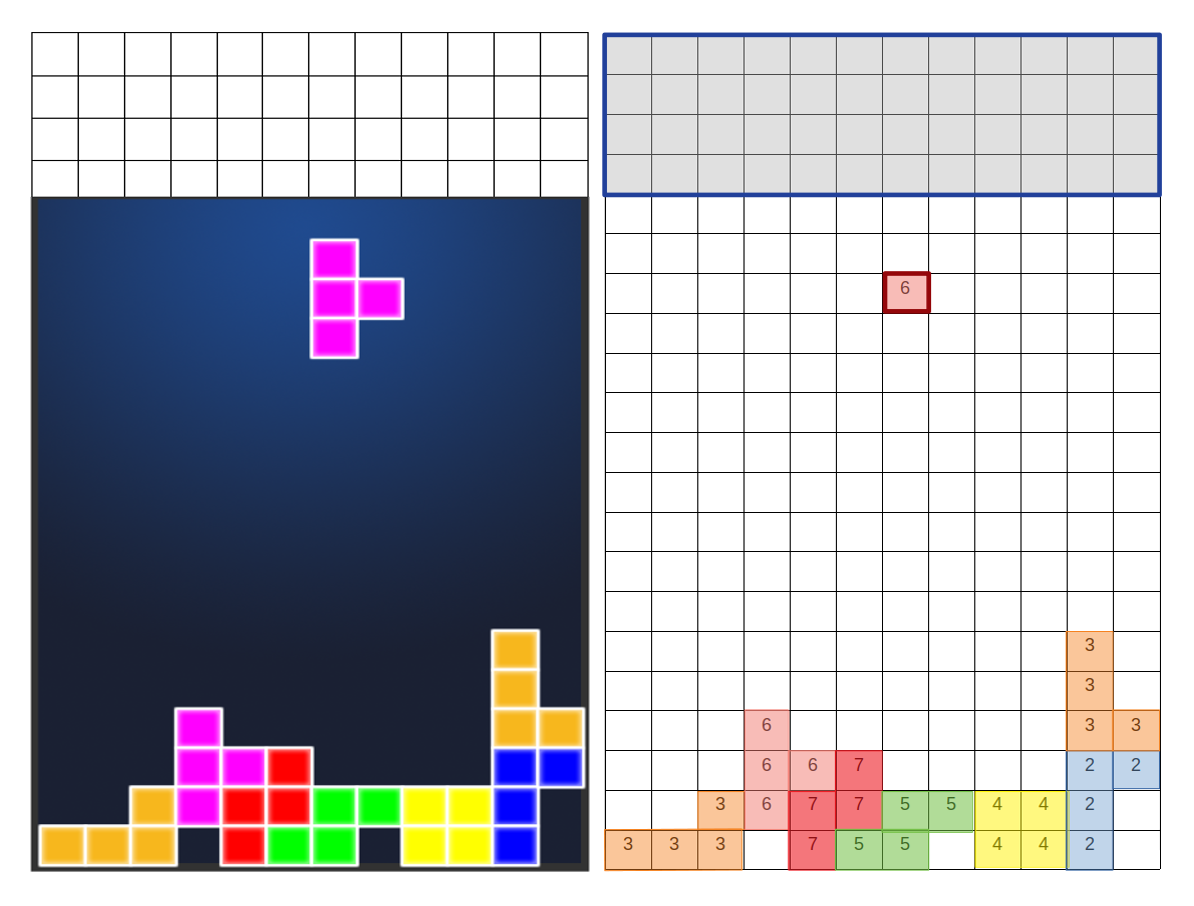
\includegraphics[scale=0.35]{img/grid.png}
				\caption{Représentation numérique des données dans le tableau de jeu}
				\label{fig:grid}
			\end{figure}


		\subsubsection{La fenêtre graphiques}

			\begin{figure}[bt]
				\centering
				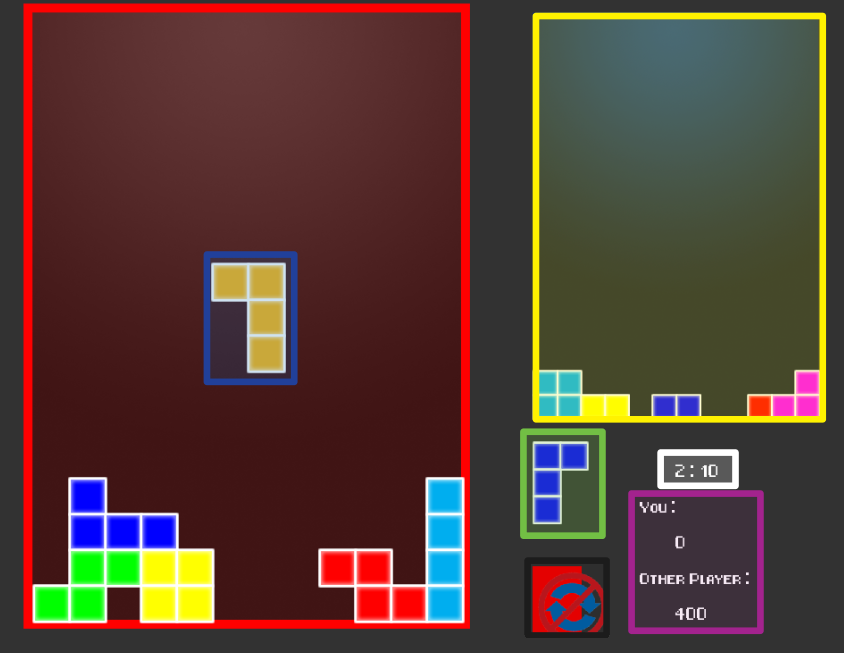
\includegraphics[scale=0.35]{img/fenetre.png}
				\caption{Différentes zone d'affichage de la fenêtre du jeu}
				\label{fig:fen}
			\end{figure}




		\subsubsection{Les actions du joueur}

			Lors de la chute du tetromino en jeu, le joueur peu intéragir sur celui ci avec les touche du clavier :

			Les flèches gauche et droite et les touche Q et D permettent de déplacer latéralement le tétromino.
			La flèche du bas et la touche S permettent d’accélérer la chute si on reste appuyé dessus.
			La barre d’espace permet de faire tourné le tetromino sur lui même.

			De plus, la fermeture de la fenêtre étant aussi une action du joueur sur le jeu, elle fait partie de la liste des contrôle.


			Pour capter les actiosn réalisés par le joueur nous avons crée une classe Controls.

			Dans cette classe nous définissons des objets de classe Action de GF.

			Pour les actions lié à une touche de clavier nous utilisons la fonction gf::Action ::addScancodeKeyControl avec le gf::Scancode correspondant à la touche voulue.

			Nous avons aussi une fonction reset qui permet de stoppé toute les actions en cours. Nous l’utilisons dans la boucle de jeu.

			+ d’explication sur le fonctionnement des classe Action et Event ?

		
	

\section*{Conclusion}


\end{document}